\subsubsection{19.01.15}
\begin{enumerate}
	
	\item Время начала и окончания собрания: 17:30 - 21:00.
	
	\item Цели собрания: 
	\begin{enumerate}
		
		\item Продолжить работу над программами автономного периода.
		
	\end{enumerate}

	\item Проделанная работа:
	\begin{enumerate}
		
		\item Сегодня все занятие было посвящено написанию автономного периода и поэтому тренировок сегодня не было.
		
		\item Передний правый привод колеса был заменен на аналогичный привод с энкодером (после установки на привод энкодер нельзя снять, поэтому пришлось менять привод целиком). Теперь у нас есть по одному рабочему энкодеру с каждой стороны робота.
		
		\item Мы решили пока не исключать возможность написания программы автономного периода по ИК-датчику, однако было решено отложить это на более позднее время. Идея же программы автономного периода без ИК-датчика претерпела некоторые изменения:  Съехать с пандуса, забросить маленький мяч в подвижную корзину высотой 60 см и захватить ее. Повернуться против часовой стрелки и отпустить корзину 60 см так, чтобы она оказалась на прямой, соединяющей корзину 90 см и зону парковки. Повернуться обратно по часовой стрелке, подъехать к корзине 90 см, захватить ее и забросить в нее большой мяч. Двигаясь в зону парковки с корзиной 90 см параллельно толкать перед собой корзину 60 см. Заехать в зону вместе с корзинами. (Максимум 140 очков). Программа движения была написана, забрасывание мячей в подвижные корзины будет реализовано позднее, когда у нас в распоряжении будут оригинальные корзины.
		
		\item Для того, чтобы закидывать в корзину первый автономный шарик, нами был разработан специальный крючок. Чтобы мяч высвободился из крючка, необходимо слегка надавить на него снизу. Поэтому он не выпадает во время движения, а для закидывания его в корзину нужно подъехать к ней вплотную и начать опускать подъемник: в тот момент, когда мячик коснется стенки подвижной корзины, он высвободится и упадет в нее.
        \begin{figure}[H]
	  	  \begin{minipage}[h]{0.2\linewidth}
	  	    \center  
	  	  \end{minipage}
	  	  \begin{minipage}[h]{0.6\linewidth}
	  		\center{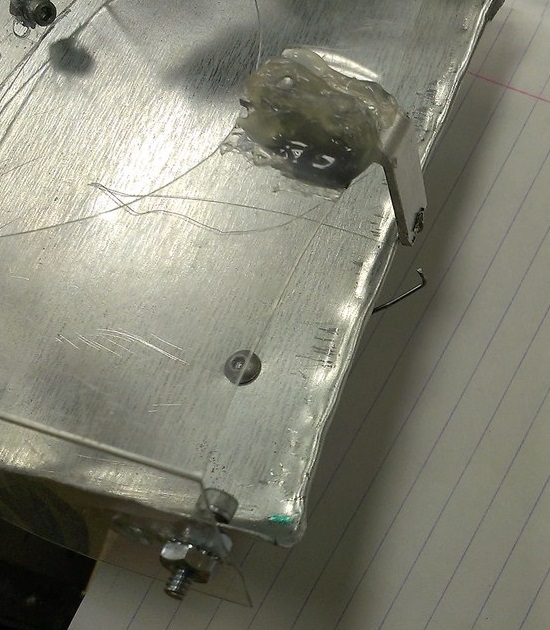
\includegraphics[scale=0.3]{days/19.01.15/images/01}}
	  	  \end{minipage}
	  	  \caption{Крючок длоя автономного мяча}
	   \end{figure} 
	   
	   \item Было замечено, что средняя пара реек проваливается вниз, когда подъемник находится в сложенном состоянии. Для того, чтобы это исправить, сверху реек были установлены дополнительные ограничители.
	   \begin{figure}[H]
	   	\begin{minipage}[h]{0.2\linewidth}
	   		\center  
	   	\end{minipage}
	   	\begin{minipage}[h]{0.6\linewidth}
	   		\center{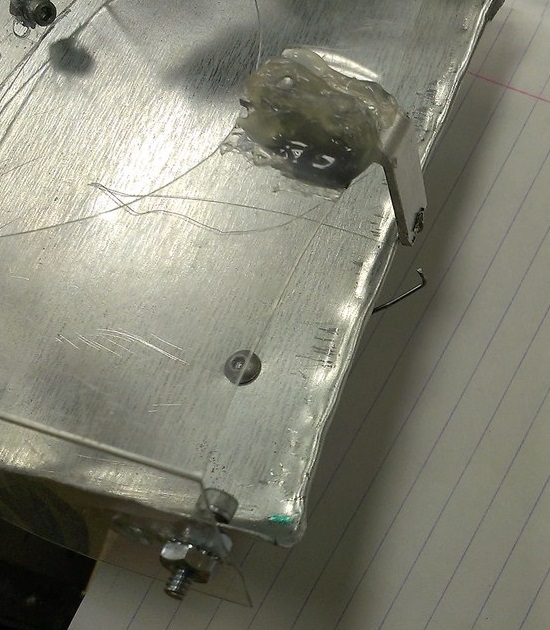
\includegraphics[scale=0.3]{days/19.01.15/images/01}}
	   		\caption{Ограничители хода реек}
	   	\end{minipage}
	   \end{figure}

	\end{enumerate}
	
	\item Итоги собрания:
	\begin{enumerate}
		
		\item Измененная программа автономного периода при старте с пандуса частично написана.
		
		\item На переднем правом приводе теперь есть энкодер.
		
        \item Установлены ограничители хода реек.
		
	\end{enumerate}
	
	\item Задачи для последующих собраний:
	\begin{enumerate}
		
		\item Написать программу автономного периода при старте из зоны парковки.
		
		\item Продолжить тренировки.
			
	\end{enumerate}
\end{enumerate}
\fillpage
